\subsection{Robot Kinematics [MH]}
In this chapter, both the direct and the inverse kinematics are presented.
The direct kinematics is used for calculating the initial offset between endeffector
and head and for performing the hand-eye calibration. The inverse kinematics is used to
move the robot.
\subsubsection{Direct Kinematics}
The Denavit-Hartenberg (DH) parameters of the UR3 robot are depicted in Fig.~\ref{fig1}.
\begin{figure}[htbp]
\centerline{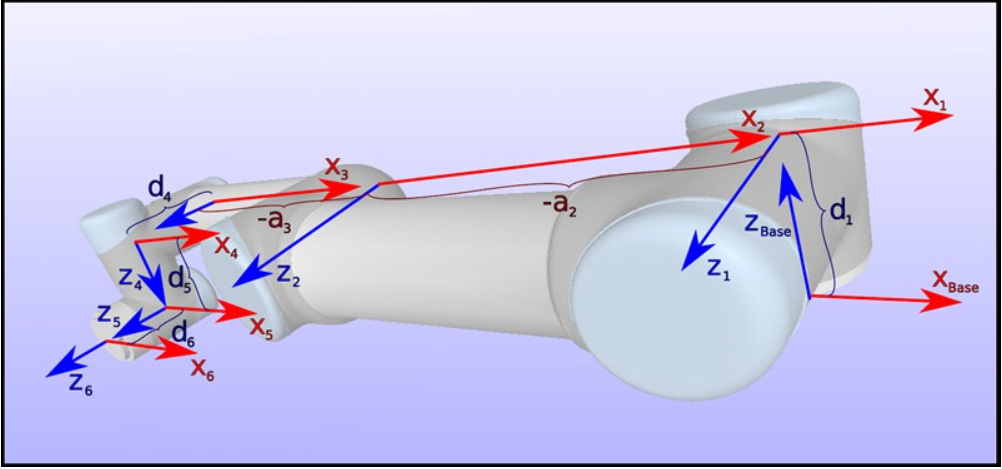
\includegraphics[width=8cm]{DH}}
\caption{DH parameters of the UR3.}
\label{fig1}
\end{figure}

By using the DH convention, the DH parameters can be obtained as shown in table \ref{tab1}.

\begin{table}[htbp]
\caption{DH parameters of the UR3 robot}
\begin{center}
\begin{tabular}{|c|c|c|c|c|}
\hline
\cline{2-5} 
\textbf{joint} & \textbf{\textit{$\theta_{i}$ [deg]}}& \textbf{\textit{$a_{i}$ [m]}}& \textbf{\textit{$d_{i}$ [m]}} & \textbf{\textit{$\alpha_{i}$ [deg]}}\\
\hline
i = 1& $\theta_{1}$& 0& 0.1519& 90 \\
i = 2& $\theta_{2}$& -0.24356& 0& 0 \\
i = 3& $\theta_{3}$& -0.21325& 0& 0 \\
i = 4& $\theta_{4}$& 0& 0.11235& 90 \\
i = 5& $\theta_{5}$& 0& 0.08535& -90 \\
i = 6& $\theta_{6}$& 0& 0.0819& 0 \\
\hline
\end{tabular}
\label{tab1}
\end{center}
\end{table}
The transformation from joint $i$ to joint $i-1$ can be calculated by \eqref{eq1}, where $s_{\alpha_{i}}$ is the short form for $\sin(\alpha_{i})$ and $c_{\alpha_{i}}$ is the short form for $\cos(\alpha_{i})$
\begin{equation}
{}^{i}{T}_{i-1} = \left( \begin{array}{rrrr}                                
c_{\theta_{i}} & -c_{\theta_{i}} \cdot s_{\theta_{i}} & s_{\alpha_{i}} \cdot s_{\theta_{i}} & a_{i} \cdot c_{\theta_{i}} \\                                               
s_{\theta_{i}} & c_{\alpha_{i}} \cdot c_{\theta_{i}} & -s_{\alpha_{i}} \cdot c_{\theta_{i}} &  a_{i} \cdot s_{\theta_{i}} \\                                               
0 & s_{\alpha_{i}} & c_{\alpha_{i}} & d_{i} \\
0 & 0 & 0 & 1 \\                                               
\end{array}\right)
\label{eq1}
\end{equation}

Using \eqref{eq1}, the forward kinematics of the UR3 robot can be calculated 
\begin{equation}
{}^{0}{T}_{6}={}^{0}{T}_{1} \cdot {}^{1}{T}_{2} \cdot {}^{2}{T}_{3} \cdot {}^{3}{T}_{4} \cdot {}^{4}{T}_{5} \cdot {}^{5}{T}_{6}
\label{eq2}
\end{equation}

\subsubsection{Inverse Kinematics}
In general, the inverse kinematics of a 6 degrees of freedom robot can’t be calculated analytically. However, with the geometry of the UR3 robot, there are rotation axes which are parallel to each other or intersecting. As a result, the inverse kinematics gets easier and in the case of the UR3, the inverse kinematics can be solved analytically. The equations and their derivations can be found in $\cite{andersen2018kinematics}$. For the joint angles $\theta_{1}$, $\theta_{3}$ and $\theta_{5}$ one can choose either a positive or a negative sign, which denotes different possibilities to move the robot to the same pose. Because the sign of one angle infuences the value of other angles, there are in general 8 different solutions for the inverse kinematics. This effect can be seen in the equation of $\theta_{5}$ which depends on $\theta_{1}$

\begin{equation}
\theta_{5}=\pm \arccos\left(\frac{{}^{0}{P}_{6x} \cdot \sin(\theta_{1})-{}^{0}{P}_{6y} \cdot \cos(\theta_{1})-d_{4}}{d_{6}}\right)
\label{eq3}
\end{equation}

However, in some constellations fewer than 8 solutions exist because a few solutions are geometrically not possible. The inverse kinematics algorithm makes sure that only the existing solutions are considered and compares them with the current robot position. The existing solution which is closest to the current robot position is then passed to the motion compensation. This solution is found by taking the squared distance of the current joint states and the actual existing solutions.
